\section{Сеточное решение уравнения Пуассона}
\subsection{Постановка задачи}

Будем рассматривать многомерное дифференциальное уравнение в области $\Omega$:
\begin{equation}
    \label{eq:poissonnd_lam}
    -\nabla\cdot\left(\lambda(\vec x)\nabla u\right) = f(\vec x), \quad \vec x \in \Omega
\end{equation}

Оператор в левой части (оператор Лапласа)
описывает физический процесс диффузии c коэффициентом диффузии $\lambda$.
Это уравнение (с нулевой правой частью) используют
в частности для расчёта распределения температуры в однородном твёрдом теле.
В этом случае коэффиент $\lambda$ называют коэффициентом теплопроводности,
а за счёт ненулевой $f$ можно задавать дополнительные
внутренние источники тепла.

В простом случае постоянного коэффициент диффузии ($\lambda = \const$) его
можно вынести из под дивергеции и отнести в правую часть. Тогда уравнение упростится до однородного вида:
\begin{equation}
    \label{eq:poissonnd}
    -\nabla^2 u = f(\vec x), \quad \vec x \in \Omega
\end{equation}

Далее на границе области расчёта $\partial \Omega$
рассмотрим несколько типов граничных условий.

\subsubsection{Граничные условия первого рода}
Также известны как граничные условия Дирихле.
На границе $\partial \Omega_{I}$ задано точное значение искомой функции $u^\Gamma$:
\begin{equation}
\label{eq:poissonnd_bc}
u = u^\Gamma(\vec x), \quad \vec x \in \partial\Omega_I
\end{equation}

В аналогии задачи теплопроводности это условие
можно трактовать как условие заданной на стенке температуры.

\subsubsection{Граничные условия второго рода}
Также известны как граничные условия Неймана.
На границе $\partial \Omega_{II}$ задано значение нормальной производной искомой функции $q$:
\begin{equation}
\label{eq:poissonnd_bc2}
-\lambda(\vec x)\dfr{u}{n} = q(\vec x), \quad \vec x \in \partial\Omega_{II}
\end{equation}

В аналогии задачи теплопроводности это условие можно трактовать как условие заданного на стенке теплового потока.

\subsubsection{Граничные условия третьего рода}
Также известны как граничные условия Робэна.
На границе $\partial \Omega_{III}$ задано линейное соотношение значений функции и нормальной производной:
\begin{equation}
\label{eq:poissonnd_bc3}
-\lambda(\vec x)\dfr{u}{n} = \alpha(\vec x) u + \beta(\vec x), \quad \vec x \in \partial\Omega_{III}.
\end{equation}

При постановке задачи теплопроводности это условие часто записывают в виде
$$
-\lambda(\vec x)\dfr{u}{n} = \alpha(\vec x)\left(u - u^0\right).
$$
где известное значение $u^0$ называют температурой окружающей стреды.
Такое условие называют условием конвективной теплопроводности или условием Ньютона--Рихмана.
Для приведения этого условия к исходному виду \cref{eq:poissonnd_bc3} достаточно положить $\beta = -\alpha u^0$.

\subsubsubsection{Об универсальности условий третьего рода}
Условия \cref{eq:poissonnd_bc,eq:poissonnd_bc2}
можно свести к условиям \cref{eq:poissonnd_bc3}
при правильном подборе коэффициентов $\alpha$ и $\beta$.
Так для условий второго рода нужно положить $\alpha=0$, $\beta=q$.
А для условий первого рода: $\alpha=\eps^{-1}$, $\beta = -\alpha u^\Gamma$,
где $\eps\to 0$ -- некоторое очень малое положительное число.

\subsubsection{Периодические граничные условия}
Необходимость в таких условиях
возникает при расчёте физических процессов
около периодических структур: решёток, лопастей, рядов скважин, оребрения нагревателя и т.п.
В этом случае из исходную большую область расчёта
представляют как бесконечную последовательность однотипных ячеек периодичности, 
в каждой из которых решения полностью идентичны (в более сложных вариантах -- сдвинуты на константу).

\begin{figure}[h!]
\centering
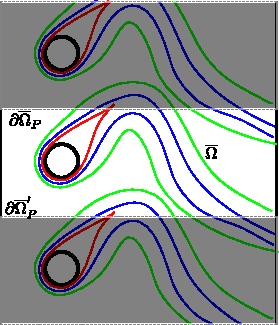
\includegraphics[width=0.4\linewidth]{periodic_bc.pdf}
\caption{Ячейка периодичности в задаче обтекания бесконечной решётки}
\label{fig:periodic_bc}
\end{figure}
На \figref{fig:periodic_bc} представлен пример области с выделенной ячейкой периодичности $\overline\Omega$ (незатенённая область).
Изолинии можно трактовать как изотермы решения задачи о нестационарном обтекании решётки нагревателя
(поле температур в этом случае описывается более сложным уравнением, чем \cref{eq:poissonnd_lam}
и приведено тут только для иллюстрации периодичности).

Пара периодических границ обозначена через $\partial\overline\Omega_P$ и $\partial\overline\Omega_P'$.
Пусть эти границы топологически экваивалентны, то есть для любой точки $\vec x\in\partial\overline\Omega_P$
cуществует взаимноодносзначная точка $\vec x'\in\partial\overline\Omega_P'$.
Для того, чтобы решение за этими границами точно соответствовало решению внутри ячейки периодичности необходимо
задать равенство значений и производных любого порядка:
\begin{equation}
\label{eq:poissonnd_bcp}
\left\{
\begin{array}{l}
    u(\vec x) = u(\vec x'), \\ [10pt]
    \left.\displaystyle\frac{\partial^k u}{\partial n^k}\right|_{\vec x} = -\left.\displaystyle\frac{\partial^k u}{\partial n^k}\right|_{\vec x'}
\end{array}
\right.
\vec x\in\partial\overline\Omega_P, \quad \vec x'\in\partial\overline\Omega_P', \quad \forall k.
\end{equation}
Здесь под $n$ подразумевается внешняя к ячейке периодичности нормаль, поэтому в правой части
условия для производных стоит минус.



\subsection{Метод конечных разностей}
Рассмотрим задачу \cref{eq:poissonnd,eq:poissonnd_bc} в упрощённой одномерной постановке:
\begin{equation}
    \label{eq:poisson1d}
    -\ddfrq{u}{x} = f(x)
\end{equation}
в области $x\in[a,b]$ с граничными условиями первого рода
\begin{equation}
	\label{eq:poisson1d_bc}
	\begin{cases}
        u(a)=u_a,\\[5pt]
        u(b)=u_b.\\
	\end{cases}
\end{equation}

Необходимо:
\begin{itemize}
\item 
	Запрограммировать расчётную схему для численного решения этого уравнения методом конечных разностей
	на сетке с постоянным шагом,
\item
	С помощью вычислительных экспериментов подтвердить порядок аппроксимации расчётной схемы.
\end{itemize}

\subsubsection{Метод решения}

\subsubsubsection{Нахождение численного решения}

В области решения $[a,b]$ введём равномерную сетку из $N$ ячеек.
Шаг сетки будет равен $h=(b-a)/N$.
Узлы сетки запишем в виде сеточного вектора $\{x_i\}$ длины $N+1$, где $i=\overline{0,N}$.
Определим сеточный вектор $\{u_i\}$ неизвестных, элементы которого определяют значение искомого численного решения в $i$-ом узле сетки. 

Разностная схема второго порядка для уравнения \eqref{eq:poisson1d} имеет вид
\begin{equation}
    \label{eq:poisson1d_fdm}
    \frac{-u_{i-1} + 2u_{i} - u_{i+1}}{h^2} = f_i, \qquad i=\overline{1,N-1}.
\end{equation}
Здесь $\{f_i\}$ -- известный сеточный вектор, определяемый через известную
аналитическую функцию $f(x)$ в правой части уравнения \eqref{eq:poisson1d} как
\begin{equation}
    \label{eq:poisson1d_fdm2}
    f_i = f(x_i).
\end{equation}

Аппроксимация граничных условий \eqref{eq:poisson1d_bc} первого рода даёт дополнительные 
сеточные уравнения для граничных узлов
\begin{equation}
    \label{eq:poisson1d_fdm_bc}
    \begin{array}{ll}
        u_0 = u_a,\\
        u_N = u_b
    \end{array}
\end{equation}

Линейные уравнения \eqref{eq:poisson1d_fdm}, \eqref{eq:poisson1d_fdm_bc}
составляют систему вида

\begin{equation*}
    \sum_{j=0}^{N} A_{ij}\,u_j = b_i, \qquad i=\overline{0,N}
\end{equation*}
с матричными коэффициентами
\begin{equation}
    \label{eq:poisson1d_fdm_lhs}
    A_{ij} = \begin{cases}
        1,      &\quad i=0, \, j=0; \\
        2/h^2,  &\quad i=\overline{1,N-1}, \, j=i;\\
        -1/h^2, &\quad i=\overline{1,N-1}, \, j=i-1;\\
        -1/h^2, &\quad i=\overline{1,N-1}, \, j=i+1;\\
        1,      &\quad i=N, \, j=N; \\
        0,      &\quad \text{иначе}.
    \end{cases}
\end{equation}
и правой частью
\begin{equation}
    \label{eq:poisson1d_fdm_rhs}
    b_i = \begin{cases}
        u_a,   &\quad i=0;\\
        u_b,   &\quad i=N;\\
        f_i,   &\quad i=\overline{1,N-1}.
    \end{cases}
\end{equation}
Искомый вектор находится путём решения этой системы.

\subsubsubsection{Практическое определения порядка аппроксимации}
\label{sec:compute-appr}

Порядок аппрокцимации показывает скорость
приближения численного решения к точному с уменьшением сетки.
Поэтому для подтверждения порядка необходимо
\begin{itemize}
\item Знать точное решение,
\item Уметь вычислять функционал (норму, $||\cdot||$), характеризующий отклонение точного решения от численного,
\item Сделать несколько расчётов на сетках с разной $N$  и заполнить таблицу $||\{u_i - u^e(x_i)\}||(N)$,
\item На основе этой таблицы построить график в логарифмических осях и по углу наклона кривой сделать вывод о порядке аппроксимации.
\end{itemize}

Выберем произвольную функцию $u^e$ (достаточно сильно изменяющуюся на целевом отрезке $[a,b]$).

Далее путём прямого вычисления определим параметры задачи $f$, $u_a$, $u_b$ такие,
для которых функция $u^e$ является точным решением задачи \eqref{eq:poisson1d}, \eqref{eq:poisson1d_bc}.

Зададимся числом разбиений $N$ и решим задачу для выбранным параметров.
В результате определим сеточный вектор численного решения $\{u_i\}$.

В качестве нормы выберем стандартное отклонение. В интегральном виде для многомерной функции $y(\vec x)$
в области $\vec x\in D$ оно имеет вид
\begin{equation}
    \label{eq:norm2_common}
    ||y(\vec x)||_2 = \sqrt{\frac{1}{|D|}\int_{D} y(\vec x)^2 \, d\vec x}.
\end{equation}
Упрощая до одномерного случая
\begin{equation*}
    ||y(x)||_2 = \sqrt{\frac{1}{b-a}\int_{a}^{b} y(x)^2 \, dx}.
\end{equation*}

Вычислим этот интеграл численно на введённой ранее равномерной сетке $\{x_i\}$:
\begin{equation*}
    ||\{y_i\}||_2 = \sqrt{\frac{1}{b-a}\sum_{i=0}^{N} w_i y_i^2},
\end{equation*}
где $\{w_i\}$ -- вес (или "площадь влияния") $i$-ого узла:
\begin{equation*}
    w_i = \begin{cases}
        h/2, &\quad i=0, N;\\
        h, &\quad i=\overline{1,N-1},
    \end{cases}
\end{equation*}
такая что
\begin{equation*}
    \sum_{i=0}^{N} w_i = b-a.
\end{equation*}

Окончательно среднеквадратичная норма отклонения численного решения от точного запишется в виде
\begin{equation}
    \label{eq:poisson1d_fdm_norm}
    ||\{u_i - u^e(x_i)\}||_2 = \sqrt{\frac{1}{b-a}\sum_{i=0}^{N} w_i \left(u_i - u^e_i\right)^2}.
\end{equation}

\subsubsection{Программная реализация}
\label{sec:poisson1d_prog}

\clisting{open}{"test/poisson_fdm_test.cpp"}

Тестовая программа для решения одномерного уравнения Пуассона 
реализована в файле \ename{poisson_fdm_solve_test.cpp}.

В качестве аналитической тестовой функции  используется
\begin{equation*}
    u^e = \sin(10 x^2)
\end{equation*}
на отрезке $x\in[0,1]$.

\subsubsubsection{Функция верхнего уровня}
объявлена как
\clisting{line}{", \"[poisson1-fdm]\")"}
В программе в цикле по набору разбиений \cvar{n_cells}
\clisting{line}{"for (size_t n_cells"}
создаётся решатель для тестовой задачи, использующий заданное число ячеек
\clisting{line}{"worker"}
вычисляется среднеквадратичная норма отклонения численного решения от точного
\clisting{line}{"n2"}
полученное численное решение (вместе с точным) сохраняется в vtk файле\\
\ename{poisson1_n={10,20,...}.vtk}
\clisting{line}{"save_vtk"}
а полученная норма печатается в консоль напротив количества ячеек
\clisting{line}{"cout"}

В результате работы программы в консоли должна отобразиться таблица вида
\begin{shelloutput}
--- [poisson1] ---
10 0.179124
20 0.0407822
50 0.00634718
100 0.00158055
200 0.000394747
500 6.31421e-05
1000 1.57849e-05
\end{shelloutput}
где первый столбец -- это количество ячеек, а второй -- полученная для этого количества ячеек норма.
Нарисовав график этой таблицы в логарифмических осях подтвердим второй порядок аппроксимации (\figref{fig:poisson_convergence}).

\begin{figure}[h]
\centering
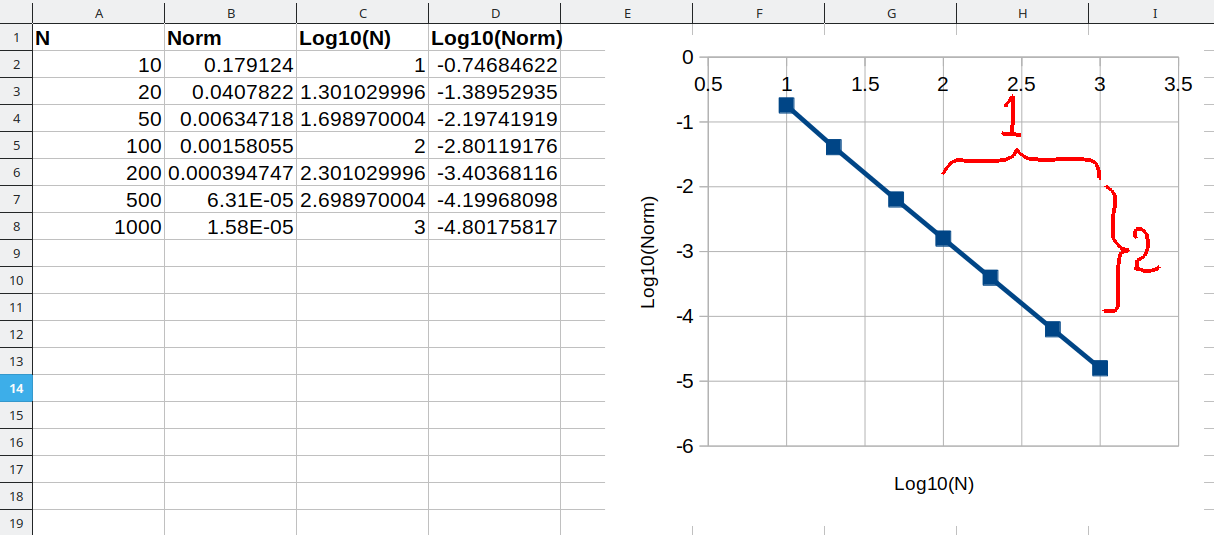
\includegraphics[width=0.9\linewidth]{poisson1_appr.png}
\caption{Сходимость с уменьшением разбиения при решении одномерного уравнения Пуассона}
\label{fig:poisson_convergence}
\end{figure}

Открыв один из cохранённых в процессе работы файлов vtk \ename{poisson1_ncells=?.vtk} в paraview
можно посмотреть полученные графики. В файле представлены как точное ``exact'', так и численное решение ``numerical''
(\figref{fig:poisson_graph}).

\begin{figure}[h]
\centering
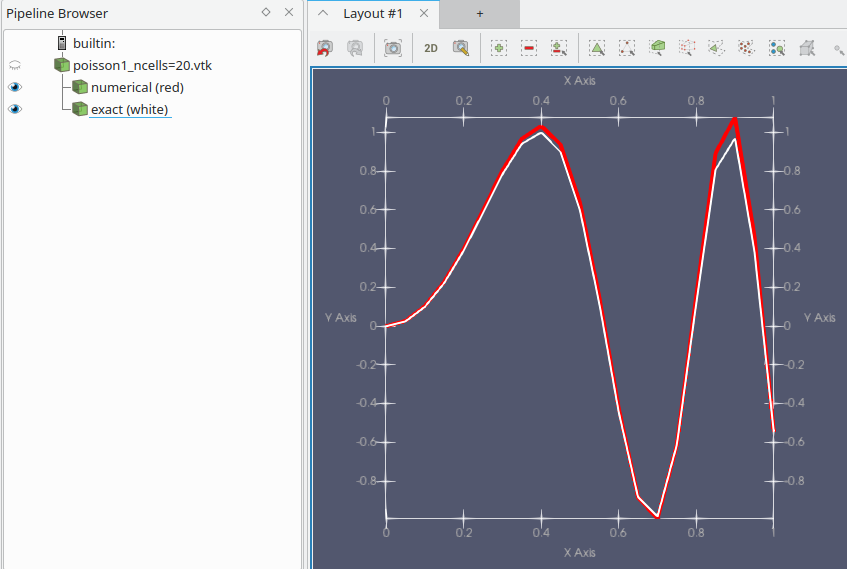
\includegraphics[width=0.9\linewidth]{poisson1_graph.png}
\caption{Сравнение точного и численного решений уравнения Пуассона}
\label{fig:poisson_graph}
\end{figure}


\subsubsubsection{Детали реализации}
\clisting{open}{"test/poisson_fdm_test.cpp"}
Основная работа по решению задачи проводится в классе \cvar{TestPoisson1Worker}.

В его конструкторе происходит инициализация сетки (приватного поля класса) на отрезке $[0, 1]$ с заданным разбиением
\cvar{n_cells}:
\clisting{line}{"TestPoisson1Worker"}

В методе \cvar{solve()} производится численное решения задачи и вычисления нормы.
Для этого последовательно
\begin{enumerate}
\item Строится матрица левой части и вектор правой части определяющей системы уравнений.
      Матрицы хранятся в разреженном формате CSR (\secref{sec:csr}), удобном для последовательного чтения.
\item Вызывается решатель СЛАУ. Решение записывается в приватное поле класса \cvar{u}.
\item Вызывается функция вычисления нормы.
\end{enumerate}

\clisting{block}{"double solve()"}

Функции нижнего уровня (используемые в методе \cvar{solve}):
\begin{itemize}
\item
  Сборка левой части СЛАУ. Реализует формулу \eqref{eq:poisson1d_fdm_lhs}.
  Для заполнения матрицы используется формат \cvar{cfd::LodMatrix} (\secref{sec:lodmat}), удобный для непоследовательной записи, который в конце конвертируется CSR.
  \clisting{block}{"approximate_lhs("}
\item
  Сборка правой части СЛАУ. Реализует формулу \eqref{eq:poisson1d_fdm_rhs}.
  \clisting{block}{"approximate_rhs("}
\item
  Вычисление нормы. Реализует формулу \eqref{eq:poisson1d_fdm_norm}.
  \clisting{block}{"compute_norm2"}
\end{itemize}

\subsection{Метод конечных объёмов}
\label{sec:FVM}
Будем рассматривать задачу в многомерной постановке \cref{eq:poissonnd,eq:poissonnd_bc}.

\subsubsection{Конечнообъёмная сетка}
Разобъём oбласть численного решения на непересекающиеся подобласти $E_i$, $i = \overline{0, N-1}$,
а её границу $\partial \Omega$ на грани $\Gamma_s$, $s = \overline{0, N^\Gamma - 1}$ (\figref{fig:fvm_grid}).
Введем следующие сеточные примитивы:
\begin{itemize}
\item $E_i$ -- ячейка сетки,
\item $\Gamma_{s}$ -- граничная грань,
\item $\vec c_i$ -- центр (масс) ячейки,
\item $\vec g_s$ -- центр (масс) грани $\Gamma_{s}$,
\item $\gamma_{ij}$ -- внутренняя грань между $i$-ой и $j$-ой ячейками,
\end{itemize}
Будем считать, что ячейки сетки выпуклые, а грани -- плоские.

\begin{figure}[h!]
\centering
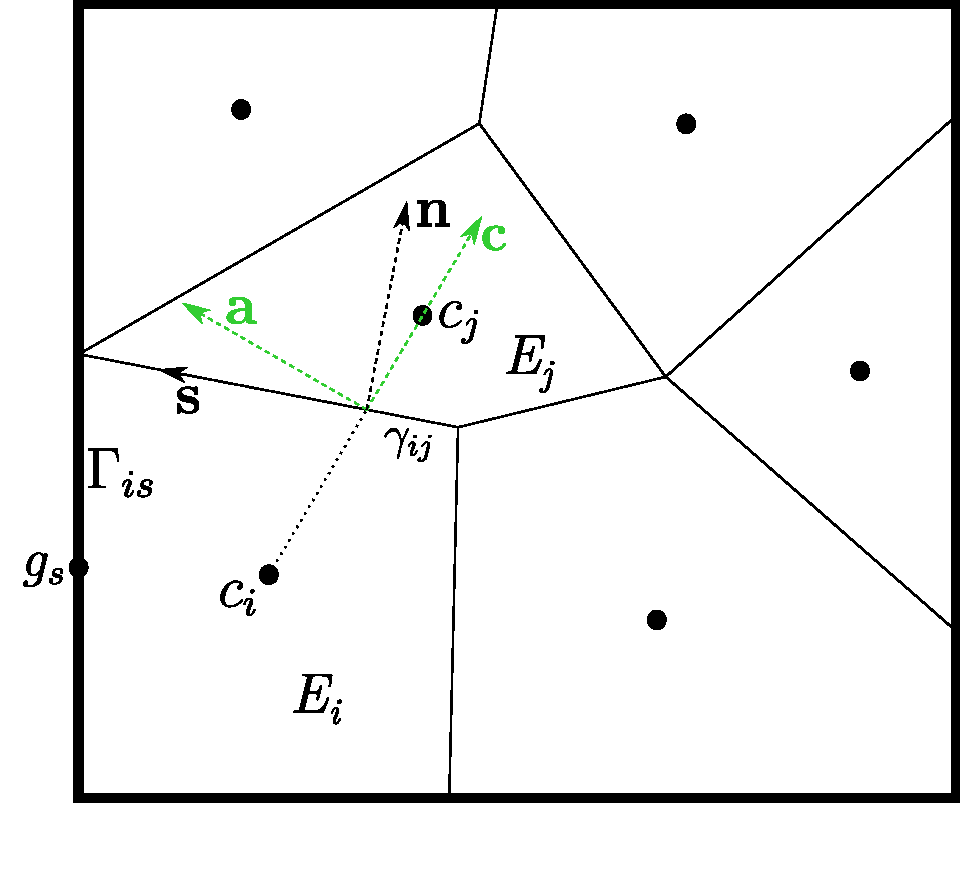
\includegraphics[width=0.4\linewidth]{fvm_grid.pdf}
\caption{Конечнообъёмная сетка}
\label{fig:fvm_grid}
\end{figure}

\subsubsection{Конечнообъёмная аппроксимация}
\label{sec:fvm_appr}

Проинтегрируем исходное уравнение по одной из подобластей $E_i$:
\begin{equation*}
-\arint{\nabla^2 u}{E_i}{s} = \arint{f}{E_i}{\vec x}.
\end{equation*}
К интегралу в левой части применим формулу интегрирования по частям \cref{eq:partint_laplace}. Получим
\begin{equation}
\label{eq:fvm_pois_int}
-\arint{\dfr{u}{n}}{\partial E_i}{\vec x} = \arint{f}{E_i}{\vec x}.
\end{equation}
Здесь $\partial E_i$ -- совокупность всех границ подобласти $E_i$,
а $\vec n$ -- внешняя к подобласти нормаль.

Граница ячейки $E_i$ состоит из внутренних граней $\gamma_{ij}$ (индекс $j$ здесь
соответствует индексу соседней ячейки)
и инцидентных ей граней $\Gamma_{s}$, лежащих на внешней границе расчётной области $\Omega$.
Тогда интеграл по общей границе ячейки распишется через сумму интегралов по плоским поверхностям
$$
\arint{\dfr{u}{n}}{\partial E_i}{s} = \sum_{j\in{{\rm J}_i}}\arint{\dfr{u}{n}}{\gamma_{ij}}{s} + \sum_{s\in{\rm I}_i}\arint{\dfr{u}{n}}{\Gamma_{s}}{s}.
$$
Введены следующие обозначения множества индексов: ${\rm J}_i$ -- индексы ячеек, соседних (имеющих общую грань) с текущей ячейкой $i$,
${\rm I}_i$ -- индексы граничных граней первого рода, инцидентных ячейке $E_i$.
Аппроксимирум производную $\dsfr{u}{n}$ на каждой из граней константой.
Тогда её можно вынести из под интегралов и предыдущее выражение записать в виде
\begin{equation}
\label{eq:fvm_gamma_integral}
\arint{\dfr{u}{n}}{\partial E_i}{s} \approx
\sum_{j\in{{\rm J}_i}}
    \left|
        \gamma_{ij}
    \right|
    \left(
        \dfr{u}{n}
    \right)_{\gamma_{ij}}
+\sum_{s\in{{\rm I}_i}}
    \left|
        \Gamma_{s}
    \right|
    \left(
        \dfr{u}{n}
    \right)_{\Gamma_{s}}
\end{equation}

Аналогично, анализируя интеграл правой части \cref{eq:fvm_pois_int},
приблизим значение функции правой части $f$ внутри элемента $E_i$ константой $f_i$,
которую отнесём к центру элемента. Тогда
\begin{equation}
\label{eq:fvm_f_integral}
\arint{f}{E_i}{\vec x} \approx f_i \left|E_i\right|.
\end{equation}

Сеточный вектор $\{f_i\}$ -- есть конечнообъёмная аппроксимация
функции $f(\vec x)$ на конечнообъёмную сетку.
Значения $f_i$ при аппроксимации чаще всего находятся как значения в центрах элементов
$$
f_i = f(\vec c_i).
$$
Хотя иногда может быть использовано и другое определение,
следующее из \eqref{eq:fvm_f_integral}:
$$
f_i = \frac{1}{\left| E_i \right|} \arint{f(\vec x)}{E_i}{\vec x}.
$$


\subsubsubsection{Обработка внутренних граней}
Для начала будем рассматривать сетки, в
которых вектора $\vec c$, соединяющие центры ячеек (зедёные вектора на \figref{fig:fvm_grid}),
коллинеарны (или почти коллинеарны) нормалям к граням $\vec n$.
В этом случае производную искомой функции по нормали к грани можно записать в виде
$$
\dfr{u}{n} = \dfr{u}{c}.
$$

Далее определим значения функции $u$ в точках $c_i$, $c_j$ как $u_i$, $u_j$.
Тогда значение производной $\dsfr{u}{n}$ на внутренней грани конечного объёма
может быть приближена конечной разностью
\begin{equation}
\label{eq:fvm_dudn_dudc}
\left(\dfr{u}{n}\right)_{\gamma_{ij}} \approx \dfr{u}{c} \approx \frac{u_j - u_i}{h_{ij}}, \quad h_{ij} = |\vec c_j - \vec c_i|.
\end{equation}

Определим pebi (perpendicular-bisector) сетки как сетки, удовлетворяющие следующим свойствам
\begin{itemize}
\item линии, соединяющие центры двух соседних ячеек, перпендикулярны грани между этими ячейками;
\item внутренние грани делят линии, соединящие центры соседних ячеек, пополам.
\end{itemize}
Очевидно, что равномерная структурированная сетка удовлетворяет этим свойствам.
Для построения неструктурированных pebi-сеток используют алгоритмы построения ячеек Вороного.
Для pebi-сеток разностная схема \eqref{eq:fvm_dudn_dudc}
является симметричной разностью и, поэтому, имеет второй порядок аппроксимации.

\subsubsubsection{Учёт граничных условий первого рода}
Для вычисления второго слагаемого в правой части 
\cref{eq:fvm_gamma_integral}
следует расписать значение нормальной 
к границе производной вида
$$
\left(\dfr{u}{n}\right)_{\Gamma_{s}}.
$$
Это делается с помощью граничных условий.

Пусть в центре $\vec g_s$ грани $\Gamma_{s}$ задано 
значение искомой функции \cref{eq:poissonnd_bc}:
\begin{equation}
\label{eq:fvm_bc1}
u(\vec g_s) = u^\Gamma_s.
\end{equation}
Аппроксимацию производных
будем проводить из тех же соображений, которые использовали
при анализе внутренних граней. Только вместо центра соседнего элемента
$c_j$ будем использовать центр грани $g_s$.
В первом приближении, отбрасывая касательные производные, придём к формуле, аналогичной \cref{eq:fvm_dudn_dudc}:
\begin{equation}
\label{eq:fvm_bc1_approx}
\left(\dfr{u}{n}\right)_{\Gamma_s} \approx \frac{u^\Gamma_s - u_i}{h^\Gamma_{is}}, \quad h^\Gamma_{is} = \left| \vec g_s  - \vec c_i \right|.
\end{equation}

\subsubsection{Одномерный случай}
Рассмотрим результат конечнообъёмной аппроксимации
задачи \cref{eq:poissonnd} в одномерном случае \cref{eq:poisson1d}
на равномерной сетке с шагом $h$ (\figref{fig:fvm_grid1d}).

\begin{figure}[h!]
\centering
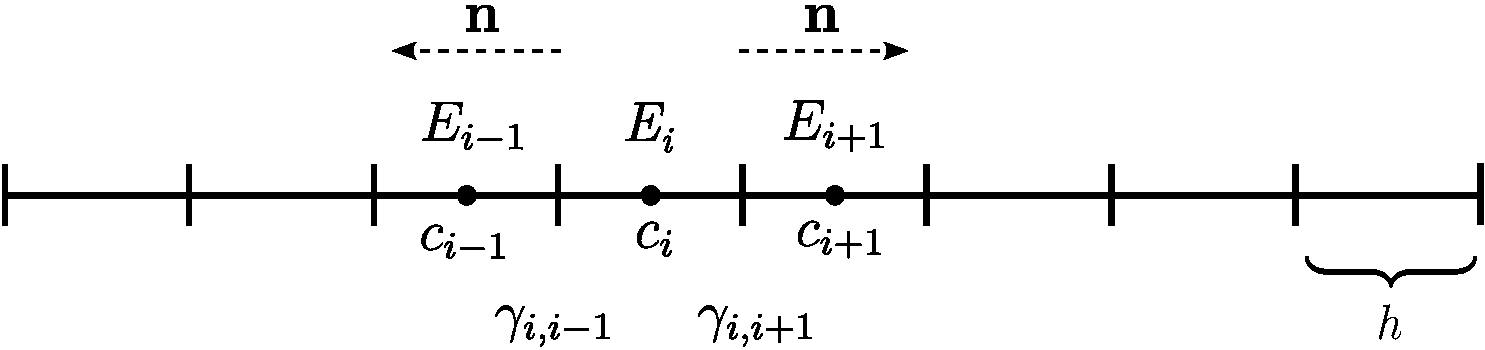
\includegraphics[width=0.6\linewidth]{fvm_grid1d.pdf}
\caption{Одномерная конечнообъёмная сетка}
\label{fig:fvm_grid1d}
\end{figure}

У внутренней ячейки $i$ есть две границы: $\gamma_{i,i-1}$ и $\gamma_{i,i+1}$.
Нормали по этим границам аппроксимируются по формулам \cref{eq:fvm_dudn_dudc}:
\begin{align*}
\gamma_{i,i-1}: \quad& \dfr{u}{n} = \frac{u_{i-1}-u_{i}}{h} \\[10pt]
\gamma_{i,i+1}: \quad& \dfr{u}{n} = \frac{u_{i+1}-u_{i}}{h}
\end{align*}
Объём ячейки в одномерном случае равен её длине $h$.
Площадь грани следует положить единице с тем, чтобы
$$
|E_i| = |\gamma| h = h.
$$
Тогда, подставляя эти значения в \cref{eq:fvm_pois_int},
получим знакомую конечноразностную схему аппроксимацию уравнения Пуассона
$$
\frac{-u_{i-1} + 2 u_i - u_{i+1}}{h} = f_i h,
$$
которая имеет второй порядок точности.
Разница с методом конечных разностей здесь состоит в том,
что значения сеточных векторов $\gvec{u}$, $\gvec{f}$ здесь
приписаны к центрам ячеек, а не к их узлам.
Это отличие проявит себя в аппроксимации граничных условий.
Так, если на левой границе $x=a$ задано условие первого рода, то соответствующее уравнение
согласно \cref{eq:fvm_bc1_approx}
примет вид
$$
-\frac{u^\Gamma_a - u_0}{h/2} - \frac{u_1 - u_0}{h} = f_0 h.
$$
В методе конечных разностей это условие выразилось бы в виде $u_0 = u^\Gamma_a$.

\subsubsection{Сборка системы линейных уравнений}
Подставим все полученные аппроксимации
\cref{eq:fvm_dudn_dudc,eq:fvm_bc1_approx}
в уравнение \cref{eq:fvm_pois_int}. Получим $i$-ое уравнение искомой системы уравнений относительно неизвестных $u_i$:
\begin{equation*}
-\sum_{j\in {\rm J}_i}
    \frac{|\gamma_{ij}|}{h_{ij}}
         \left(u_j - u_i\right)
-\sum_{s\in{\rm I}_i}
    \frac{|\Gamma_{s}|}{h^\Gamma_{is}}
        \left(u^\Gamma_s - u_i\right)
=
f_i |E_i|.
\end{equation*}
Здесь первое слагаемое в левой части отвечает за потоки через внутренние границы,
второе -- граничные условия первого рода.
Далее перенесём все известные значения в правую часть и окончательно
получим линейное уравнение для $i$-го конечного объёма:
\begin{equation}
\label{eq:fvm_slae}
\sum_{j\in{\rm J}_i}
    \frac{|\gamma_{ij}|}{h_{ij}}
         \left(u_i - u_j\right)
+\sum_{s\in{\rm I}_i}
    \frac{|\Gamma_{s}|}{h^\Gamma_{is}}u_i
 =
f_i |E_i|
+\sum_{s\in{\rm I}_i}
    \frac{|\Gamma_{s}|}{h^\Gamma_{is}} u_s^\Gamma
\end{equation}
Таким образом мы получили систему из $N$ (по количеству подобластей) линейных уравнений относительно
неизвестного сеточного вектора $\left\{u_i\right\}$
$$
A u = b.
$$

Полученные в результате сборочных процедур матрицы являются разреженными -- то есть большинство их элементов равно нулю.
Полное хранение таких матриц в памяти невозможно, поэтому применяют специальные процедуры разреженного хранения (см. \secref{sec:sparse-matrix}).

Ниже приведён псеводкод для сборки СЛАУ. Перед началом процедур сборки левую правую часть нужно инициализировать нулями.

\subsubsubsection{Алгоритм сборки в цикле по ячейкам}
\label{sec:poisson_fvm_cellbased}
Матрицу $A$ и правую часть $b$ системы \cref{eq:fvm_slae} можно
собирать в цикле по ячейкам: строчка за строчкой.
Такой алгоритм выглядел бы следующим образом
\begin{equation*}
\begin{array}{ll}
\textbf{for } i = \overline{0, N-1}                          & \textrm{-- цикл по строкам СЛАУ}\\
\qquad b_i = |E_i| f_i                                       & \\
\qquad \textbf{for } j \in \textrm{nei(i)}                   & \textrm{-- цикл по ячейкам, соседним с ячейкой $i$}\\
\qquad \qquad v = \sfrac{|\gamma_{ij}|}{h_{ij}}              & \\
\qquad \qquad A_{ii} \pluseq v                               & \\
\qquad \qquad A_{ij} \minuseq v                              & \\
\qquad \textbf{endfor}                                       & \\
\qquad \textbf{for } s \in \textrm{bnd1(i)}                  & \textrm{-- цикл по граням ячейки $i$ с условиями первого рода}\\
\qquad \qquad v = \sfrac{|\Gamma_{s}|}{h^\Gamma_{is}}        & \\
\qquad \qquad A_{ii} \pluseq v                               & \\
\qquad \qquad b_{i}  \pluseq u_s^{\Gamma} v                  & \\
\qquad \textbf{endfor}                                       & \\
\textbf{endfor}
\end{array}
\end{equation*}
Первым недостатком такого алгоритма является наличие вложенных циклов.
Во-вторых, коэффициент, отвечающий за поток через внутреннюю грань $\gamma_{ij}$,
равный $\sfrac{|\gamma_{ij}|}{h_{ij}}$ в таком алгоритме будет учитываться дважды:
в строке $i$ и в строке $j$.

\subsubsubsection{Алгоритм сборки в цикле по граням}
\label{sec:poisson_fvm_facebased}
Вместо общего цикла по ячейкам, будем использовать цикл по граням.
В таком цикле коэффициенты потоков будут вычисляться один раз
и вставляться сразу в две строки матрицы, соответствующие соседним с гранью ячейкам.
Вложенных циклов в такой постановке удаётся избежать, потому
что у грани есть только две соседние ячейки (в то время как у ячейки может быть произвольное
количество соседних граней).

Разделим все грани на исходной сетки на внутренние и граничные (отдельный набор для каждого вида граничных условий).
Тогда для внутренних граней можно записать
\begin{equation}
\label{eq:fvm_assem_internal}
\begin{array}{ll}
\textbf{for } s \in\textrm{internal}                     & \textrm{-- цикл по внутренним граням}\\ 
\qquad i,j = \textrm{nei\_cells(s)}                      & \textrm{-- две ячейки, соседние с текущей гранью}\\
\qquad v = \sfrac{|\gamma_{ij}|}{h_{ij}}                 & \\
\qquad A_{ii} \pluseq  v; \quad A_{jj} \pluseq  v        & \textrm{-- диагональные коэффициенты матрицы}\\ 
\qquad A_{ij} \minuseq v; \quad A_{ji} \minuseq v        & \textrm{-- внедиагональные коэффициенты матрицы}\\
\textbf{endfor}                                          & \\
\end{array}
\end{equation}
Граничные условия учитываются в отдельных циклах.
Здесь будем учитывать, что у грани, принадлежащей
границе области, есть только одна соседняя ячейка.
Условия первого рода:
\begin{equation}
\label{eq:fvm_assem_bc1}
\begin{array}{ll}
\textbf{for } s \in\textrm{bnd1}                         & \textrm{-- грани с условиями первого рода}\\ 
\qquad i = \textrm{nei\_cell(s)}                         & \textrm{-- соседняя с граничной гранью ячейка}\\
\qquad v = \sfrac{|\Gamma_{s}|}{h^\Gamma_{is}}           & \\
\qquad A_{ii} \pluseq  v                                 & \\ 
\qquad b_{i} \pluseq u_s^\Gamma v                        & \\
\textbf{endfor}                                          & \\
\end{array}
\end{equation}
Первое слагаемое в правой части
\cref{eq:fvm_slae}
учтём отдельным циклом:
\begin{equation}
\label{eq:fvm_assem_f}
\begin{array}{ll}                                         & \\
\textbf{for } i = \overline{0,N-1}                        & \textrm{-- цикл по ячейкам}\\ 
\qquad b_i \pluseq |E_i| f_i                              & \\
\textbf{endfor}                                           &
\end{array}
\end{equation}

\subsubsection{Расширенный набор точек коллокаций}
\label{sec:poisson_fvm_extended_facebased}
До сих пор мы соотносили
элементы сеточных векторов, которые получаются при аппроксимации функции на конечнообъёмную сетку,
с центрами конечных объёмов.
То есть точками коллокации служили центры объёмов,
а длина сеточных векторов (количество точек коллокации)
равнялась количеству ячеек сетки.
Для написания аппроксимационных соотношений около границ будет удобно расширить набор точек коллокаций за счёт
центров граничных граней.

Такой подход позволяет универсализировать подходы
к аппроксимации перетоков через грани.
То есть для каждой грани вмеcто использования разных алгоритмов для внутренних \cref{eq:fvm_assem_internal} и граничных \cref{eq:fvm_assem_bc1} граней, нужно использовать универсальный алгоритм
\begin{equation}
\label{eq:fvm_assem_bc_extended}
\begin{array}{ll}
\textbf{for } s \in\overline{0, N_f - 1}            & \textrm{-- цикл по всем граням}\\
\qquad i,j = \textrm{nei\_colloc(s)}                & \textrm{-- инцидентные точки коллокаций}\\
\qquad v = \sfrac{|\gamma_{ij}|}{h_{ij}}            & \\
\qquad A_{ii} \pluseq  v, \quad A_{ij} \minuseq v   & \textrm{-- $i$-ая строка}\\ 
\qquad A_{jj} \pluseq  v, \quad A_{ji} \minuseq v   & \textrm{-- $j$-ая строка}\\ 
\textbf{endfor}                                     & \\
\end{array}
\end{equation}
Отметим, что эта процедура заполняет не только строки, соответствующие внутренним коллокациям, но и строки для граничных точек.
Последние заполняются выражениями, соответствующие интегралам от нормальных производных
\begin{equation*}
-\arint{\dfr{u}{n}}{\Gamma_s}{s} \approx -\left.\dfr{u}{n}\right|_{\vec{g}_s} |\Gamma_s|\
\approx \frac{u^\Gamma_s - u_j}{h^\Gamma_{is}} |\Gamma_s|,
\end{equation*}
где $i$ -- индекс ячейки, соседний с гранью $\Gamma_s$.
Для задач с граничными условиями первого рода эти строки излишни и будут переписаны, но они окажутся
полезными позднее, при учёте других типов граничных условий.

Строки матрицы, соответствующие граничным точкам коллокации,
будут содержеть аппроксимированные граничные условия.
Так, для граней с условиями первого рода будет аппроксимироваться непосредственно выражение
\cref{eq:fvm_bc1}. Алгоритмическом виде это примет вид
\begin{equation}
\label{eq:fvm_assem_bc1_extended}
\begin{array}{ll}
\textbf{for } s \in\textrm{bnd1}                         & \textrm{-- грани с условиями первого рода}\\ 
\qquad j = \textrm{bnd\_col(s)}                          & \textrm{-- индекс точки коллокации, соответствующей грани}\\
\qquad A_{ij} = \delta_{ij}                              & \textrm{-- единичная диагональ}\\ 
\qquad b_{j} = u^\Gamma_s                                & \\
\textbf{endfor}                                          & \\
\end{array}
\end{equation}

Преимуществами такого подхода является:
\begin{itemize}
\item Более очевидный учёт граничных условий в отдельной строке СЛАУ,
\item Наличие явно выраженного граничного значения функции в сеточном векторе.
\end{itemize}

\subsubsubsection{Пример}
\begin{figure}[h]
\centering
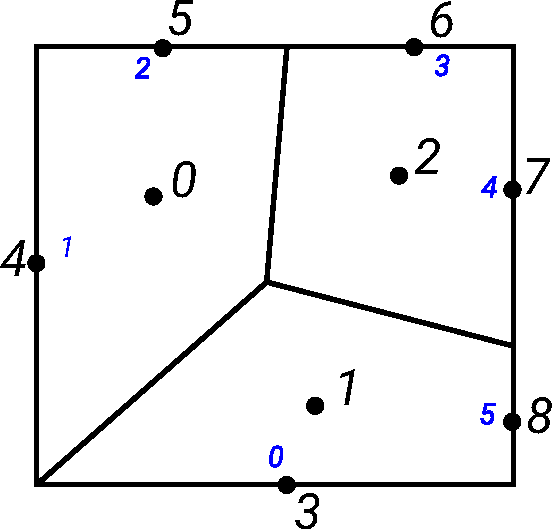
\includegraphics[width=0.25\linewidth]{extended_coll.pdf}
\caption{Расширенный набор точек коллокации}
\label{fig:extended_coll}
\end{figure}

На рис.~\ref{fig:extended_coll}.
представлена конечнообъёмная сетка, содержащая три ячейки
и девять граней. Индексация граничных граней обозначена синими цифрами.
Согласно стандартной методике конечных
объёмов сеточная функция
будет представлена массивом из трёх элементов.
В расширенном наборе будет девять точек коллокации (обозначены чёрными кругами и проиндексированы чёрными цифрами):
три соответствуют центрам ячеек и ещё шесть -- центрам граничных граней.

Пусть в области с рис.~\ref{fig:extended_coll} нужно решить
уравнение Пуассона \cref{eq:poissonnd}.
Пусть на нижней и правой гранях задано условие первого рода: $u = C$.

\paragraph{Классический подход}
Согласно классическому методу конечных объёмов
(\secref{sec:poisson_fvm_facebased})
аппроксимация задачи в ячейке с индексом 1 будет иметь следующий вид
$$
\frac{u_1 - u_0}{h_{10}}|\gamma_{10}|
+\frac{u_1 - u_2}{h_{12}}|\gamma_{12}|
+\frac{u_1 - C}{h^\Gamma_{10}}|\Gamma_0|
+\frac{u_1 - C}{h^\Gamma_{15}}|\Gamma_5|
= |E_1| f_1.
$$
Общая размерность матрицы СЛАУ при таком подходе будет
равна $3\times3$, а её элементы в 1-ой строке равны
$$
a_{10} = -\frac{|\gamma_{10}|}{h_{10}},  \quad
a_{12} = -\frac{|\gamma_{12}|}{h_{12}},  \quad
a_{11} = \frac{|\gamma_{10}|}{h_{10}}  + \frac{|\gamma_{12}|}{h_{12}} + \frac{|\Gamma_{0}|}{h^\Gamma_{10}} + \frac{|\Gamma_5|}{h^\Gamma_{15}}.
$$
Справа в 1-ой строке будет стоять
$$
b_1 = |E_1| f_1 + \frac{C |\Gamma_0|}{h^\Gamma_{10}} + \frac{C |\Gamma_5|}{h^\Gamma_{15}}.
$$

\paragraph{Новый подход}
В расширенным набором точек коллокаций
матрица правой части будет иметь размерность $9\times9$.
Из них первые три будут собираться согласно классической процедуре
метода конечных объёмов, но учитывая наличие дополнитиельных точек коллокации в центрах
граничных граней. Так, 1-ое уравнение итоговой СЛАУ, собранной согласно процедуре из
\secref{sec:poisson_fvm_extended_facebased},
примет вид
$$
\frac{u_1 - u_0}{h_{10}}|\gamma_{10}|
+\frac{u_1 - u_2}{h_{12}}|\gamma_{12}|
+\frac{u_1 - u_3}{h_{13}}|\gamma_{13}|
+\frac{u_1 - u_8}{h_{18}}|\gamma_{18}|
= |E_1| f_1.
$$
Здесь введено соотвествие для граничных граней и расстояний:
$$
\gamma_{13} = \Gamma_0, h_{13} = h^\Gamma_{10}, \gamma_{18} = \Gamma_5, h_{18} = h^\Gamma_{15}.
$$
Остальные шесть уравнений будут представлять из себя
аппроксимацию граничных условий для соответствующих граней.
Так, 3-е и 8-е уравнение будет соответствовать условию первого рода:
$$
u_3 = C, \qquad u_8 = C.
$$
Переводя рассмотренные уравнения в матричные коэффициенты, получим
следующие ненулевые коээфиициенты итоговой матрицы $\{a_{ij}\}$ и вектора правой части $\{b_i\}$. Для 1-ой строки
$$
a_{10} = -\frac{|\gamma_{10}|}{h_{10}},  \quad
a_{12} = -\frac{|\gamma_{12}|}{h_{12}},  \quad
a_{13} = -\frac{|\gamma_{13}|}{h_{13}},  \quad
a_{18} = -\frac{|\gamma_{18}|}{h_{18}},  \quad
a_{11} = a_{10} + a_{12} + a_{13} + a_{18}, \quad
b_1 = |E_1| f_1,
$$
для 3-ей строки
$$
a_{33} = 1, \quad b_3 = C,
$$
для 8-ой строки
$$
a_{88} = 1, \quad b_8 = C.
$$

\subsubsection{Граничные условия второго рода}
Рассмотрим участок границы $\partial\Omega_{II}$ на котором заданы условия второго рода
\cref{eq:poissonnd_bc2} при $\lambda=1$.
Проинтегрируем это условие по грани и получим уравнение для граничного узла коллокации:
\begin{equation*}
-\arint{\dfr{u}{n}}{\Gamma_s}{s} = \arint{q(s)}{\Gamma_s}{s} \approx |\Gamma_s| q(\vec g_s).
\end{equation*}
При сборке матрицы левой части согласно процедуре
\cref{eq:fvm_assem_bc_extended} левая часть этого уравнения уже содержит
интеграл от нормальной производной.
Тогда алгоритм сборки этого условия будет включать в себя только подстановку $q$ в правую часть:
\begin{equation}
\label{eq:fvm_assem_bc2_extended}
\begin{array}{ll}
\textbf{for } s \in\textrm{bnd2}                         & \textrm{-- грани с условиями второго рода}\\ 
\qquad j = \textrm{bnd\_col(s)}                          & \textrm{-- индекс точки коллокации, соответствующей грани}\\
\qquad b_{j} = |\Gamma_s| q(\vec g_s)                    & \\
\textbf{endfor}                                          & \\
\end{array}
\end{equation}

\subsubsection{Граничные условия третьего рода}
Теперь рассмотрим участок границы $\partial\Omega_{III}$ с условиями
\cref{eq:poissonnd_bc3} при $\lambda=1$.
Так же проинтегрируем его по $s$-ой грани
\begin{equation*}
-\arint{\dfr{u}{n}}{\Gamma_s}{s} = \arint{\alpha(s) u + \beta(s)}{\Gamma_s}{s} \approx |\Gamma_s| \left(\alpha(\vec g_s) u_s + \beta(\vec g_s)\right).
\end{equation*}
Перенесём слагаемое с неизвестной $u_s$ в левую часть (то есть добавим коэффициент в диагональ матрицы), а $\beta$ оставим справа.
Тогда, после сборки матрицы левой части по процедуре 
\cref{eq:fvm_assem_bc_extended}, модифицируем матрицу и правую часть следующим образом:
\begin{equation}
\label{eq:fvm_assem_bc3_extended}
\begin{array}{ll}
\textbf{for } s \in\textrm{bnd3}                         & \textrm{-- грани с условиями третьего рода}\\ 
\qquad j = \textrm{bnd\_col(s)}                          & \textrm{-- индекс точки коллокации, соответствующей грани}\\
\qquad A_{jj} \pluseq |\Gamma_s| \alpha(\vec g_s)             & \\
\qquad b_{j} = |\Gamma_s| \beta(\vec g_s)                & \\
\textbf{endfor}                                          & \\
\end{array}
\end{equation}

\subsubsection{Периодические граничные условия}
Рассмотрим периодическую пару границ $\partial\Omega_{P}$, $\partial\Omega_{P}'$.
Для того, чтобы такое условие можно было аппроксимировать сеточным методом,
необходимо, чтобы сетка на границе $\partial\Omega_P$ в точности соотвествовала сетке на границе $\partial\Omega_P'$.

Естественный способ удовлетворить граничные уловия вида
\cref{eq:poissonnd_bcp} -- модифицировать таблицы связности сетки так, чтобы грани, лежащие на этих границах перестали быть граничными.
То есть нужно убрать граничные точки коллокации, и добавить запись в таблицы связности \quo{грань-ячейка}.
Такая процедура требует специальной подстройки сеточных таблиц.

Чтобы этого избежать, можно работать без модификации сетки, но удовлетвормить формальным математическим условиям \cref{eq:poissonnd_bcp}.
Поскольку конечнообъёмная аппроксимация уравнения Пуассона имеет не более чем второй порядок точности, достаточно записать это условие только для первой производной.
Для периодической пары граничных граней с индексами $s$ и $s'$ это условие можно записать следующим образом:
\begin{align}
\label{eq:periodic_for_fem_poisson_1}
&u(\vec g_s) - u(\vec g_{s'}) = 0, \\
\label{eq:periodic_for_fem_poisson_2}
&-\arint{\dfr{u}{n}}{\Gamma_s}{s} - \arint{\dfr{u}{n}}{\Gamma_{s'}}{s} = 0.
\end{align}

Первое из этих условий условий запишем в строке, соответствующей грани $s$, а второе - в строке для грани $s'$.
При сборке \cref{eq:periodic_for_fem_poisson_2} учтём, что предворительно проведённая процедура
\cref{eq:fvm_assem_bc_extended}
собирает входящие в него пару интегралов в строках для грани $s$ и $s'$ соответсвенно.
Чтобы записать сумму этих интегралов, нужно просто суммировать эти строки матрицы.
Тогда процедура примет следующий вид

\begin{equation}
\label{eq:fvm_assem_bcp_extended}
\begin{array}{ll}
\textbf{for } s,s' \in\textrm{periodic\_pairs}           & \textrm{-- периодические пары граней}\\ 
\qquad i,j = \textrm{bnd\_col(s, s')}                    & \textrm{-- индексы граничных точек коллокации}\\
\qquad \textbf{for } k \in \overline{0, N+N^\Gamma-1}    & \textrm{-- цикл по столбцам}\\
\qquad\qquad  A_{jk} \pluseq A_{ik}                      & \textrm{-- складываем строки $i+j$ \cref{eq:periodic_for_fem_poisson_1}}\\
\qquad\qquad A_{ik} = 0                                  & \textrm{-- зануляем строку $i$}\\
\qquad \textbf{endfor}                                   & \\
\qquad A_{jj} \pluseq A_{ji}, \quad A_{ji} = 0           & \textrm{-- усилим диагональ $A_{jj}$ (т.к $u_i = u_j$)}\\
\qquad A_{ii} = 1, \quad A_{ij} = -1                     & \textrm{-- удовлетворим \cref{eq:periodic_for_fem_poisson_2}}\\
\textbf{endfor}                                          & \\
\end{array}
\end{equation}

\subsubsection{Учёт неортогональности сетки}
\label{sec:nonortho_fvm}
Конечнообъёмная схема, описываемая уравнениями \cref{eq:fvm_pois_int,eq:fvm_gamma_integral},
не использует в своем выводе аппроксимационных соотношений, и поэтому является точной.
Погрешность аппроксимации вносится при расписывании нормальных производных на грани
по разностным формулам: \cref{eq:fvm_dudn_dudc,eq:fvm_bc1_approx} через значения скалярной функции в точках коллокации.
Эти формулы имеют второй порядок аппроксимации в случае
ортогональных сеток. Поэтому для таких сеток
вся конечнообъёмная схема имеет второй порядок аппроксимации.
Но если в сетке присутствуют скошенные ячейки,
такие разностные соотношения дают только порядок точности.
Чтобы сохранить второй порядок для скошенных сеток необходимо 
дополнительно учитывать изменения функции поперёк нормали.

\begin{figure}[h!]
\centering
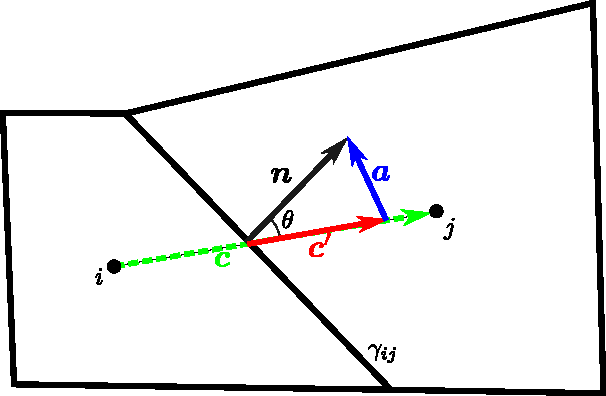
\includegraphics[width=0.4\linewidth]{skew_dfdn.pdf}
\caption{Ячейка периодичности в задаче обтекания бесконечной решётки}
\label{fig:skew_dfdn}
\end{figure}
Рассмотрим вычисление нормальной производной на грани $\gamma_{ij}$,
разделяющие точки коллокации $i$ и $j$ (\figref{fig:skew_dfdn}).
При использовании подхода с расширенным набором точек коллокации
не имеет значения, являются ли эти точки граничными коллокациями или внутренними.
Пусть вектор $\vec c$ соединяет точки коллокации.
За меру ортогональности примем значение угла $\theta$ 
между вектором единичной нормали $\vec n$ и вектором $\vec c$:
\begin{equation*}
\cos\theta = \frac{\vec n \cdot \vec c}{|\vec c|}.
\end{equation*}

Выделим некоторый вектор $\vec c'$, коллинеарный вектору $\vec c$.
И распишем вектор нормали как 
\begin{equation}
\label{eq:n_cprime_a}
\vec n = \vec c' + \vec a.
\end{equation}
Тогда
\begin{equation}
\label{eq:dudn_decomp}
\dfr{u}{n} = \nabla u \cdot \vec n = \nabla u \cdot \vec c' + \nabla u \cdot \vec a
= |\vec c'| \nabla u \cdot \frac{\vec c}{|\vec c|} + \nabla u \cdot \vec a.
\end{equation}
Первое слагаемое -- ортогональное приближение, которое 
с точностью до множителя $|\vec c'|$ равно ранее вычисленным
по разностным формулам \cref{eq:fvm_dudn_dudc,eq:fvm_bc1_approx}.
Второе -- поправка на скошенность.

Для реализации алгоритма с учётом этой поправки нужно решить следующие подзадачи:
\begin{itemize}
\item Задать длину $|\vec c'|$ (\secref{sec:cprime_a}),
\item Задать способ определения касательной производной $\nabla u\cdot \vec a$ (\secref{sec:fvm_duda}),
\item Собрать полученные соотношения в результирующую систему уравнений (\secref{sec:ortho_correction_assembly}).
\end{itemize}

\subsubsubsection{Методы разложения нормали}
\label{sec:cprime_a}
Рассмотрим различные варианты записи единичной нормали $\vec n$ в форме \cref{eq:n_cprime_a}.
Вектор $\vec c'$ сонаправлен заданному вектору $\vec c$, а вектор $\vec a$ может быть получен после определения $\vec c'$:
\begin{align*}
&\vec c' = |\vec c'| \frac{\vec c}{|\vec c|},\\
&\vec a = \vec n - \vec c'.
\end{align*}
То есть для конкретизации разложения  \cref{eq:n_cprime_a} нужно задать длину вектора $\vec c'$.
Рассмотрим три варианта её определения.

\paragraph{Поворот}

\begin{figure}[h!]
\centering
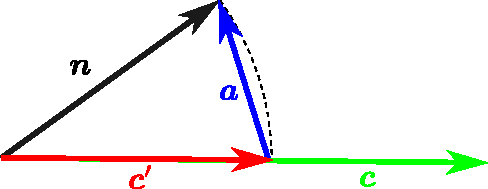
\includegraphics[width=0.4\linewidth]{cprime1.pdf}
\caption{Определение $\vec c'$ методом поворота}
\label{fig:cprime1}
\end{figure}

Положим $|\vec c'| = 1$. То есть положим длину искомого вектора равной длине единичной нормали $\vec n$ или повернём нормаль на угол $\theta$ (см. \figref{fig:cprime1}).
\begin{equation*}
\vec c' =  \frac{\vec c}{|\vec c|}.
\end{equation*}

\paragraph{Проекция}

\begin{figure}[h!]
\centering
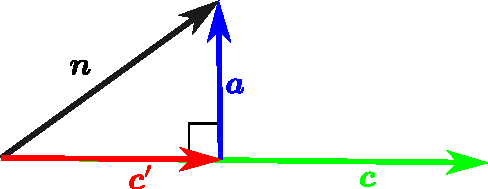
\includegraphics[width=0.4\linewidth]{cprime2.pdf}
\caption{Определение $\vec c'$ методом проекции}
\label{fig:cprime2}
\end{figure}

Определим вектор $\vec c'$ как проекцию вектора нормали на направление $\vec c$ (см. \figref{fig:cprime2}). Тогда
\begin{align*}
&|\vec c'| = \cos\theta = \frac{\vec n \cdot \vec c}{|\vec c|}, \\
&\vec c' = \frac{\vec n \cdot \vec c}{|\vec c|^2} \vec c
\end{align*}

В этом случае $|\vec c'| \leq 1$.
Таким образом, при записи нормальной производной \cref{eq:dudn_decomp} слагаемое с ортогональным приближением используется с коэффициентом, меньшим единицы.
Поэтому этот метод можно назвать методом нижней релаксации.

\paragraph{Обратная проекция}

\begin{figure}[h!]
\centering
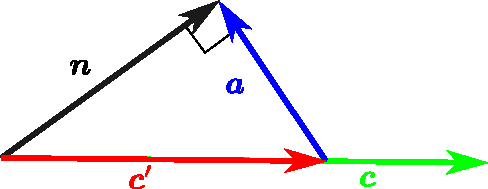
\includegraphics[width=0.4\linewidth]{cprime3.pdf}
\caption{Определение $\vec c'$ через обратную проекцию}
\label{fig:cprime3}
\end{figure}

Наоборот, опустим перпендикуляр с направления $\vec c$ на нормаль (см. \figref{fig:cprime3}):
\begin{align*}
&|\vec c'| = \frac{1}{\cos\theta} = \frac{|\vec c|}{\vec n \cdot \vec c}, \\
&\vec c' = \frac{\vec c}{\vec n \cdot \vec c}.
\end{align*}

Тогда, напротив $|\vec c'| \geq 1$, поэтому этот метод можно назвать методом верхней релаксации.
Отметим, что в этом случае вектор $\vec a$ будет параллелен грани $\gamma_{ij}$.

\subsubsubsection{Методы вычисления касательной производной}
\label{sec:fvm_duda}
Рассмотрим способы получить второе слагаемое из разложения \cref{eq:dudn_decomp}.
Напомним, что это разложение записывается для значения производной на грани конечноэлементной сетки:
\begin{equation*}
\left(\nabla u \cdot \vec a\right)_{\gamma_{ij}}
\end{equation*}
При этом функция $u$ задана своими значениями в точках коллокации, а вектор $\vec a$ известен (см. \secref{sec:cprime_a})

\paragraph{Определение через значение градиента в точках коллокации}
Пусть градиент $\nabla u$ также задан в точках коллокации.
Тогда значение на грани $\gamma_{ij}$ 
можно записать через линейную коминацию этих значений:
\begin{equation*}
\left(\nabla u\right)_{\gamma_{ij}} \approx w_i \left(\nabla u\right)_i + w_j \left(\nabla u\right)_j, \qquad w_i + w_j = 1.
\end{equation*}

Пусть $i$-ая точка коллокации граничная, тогда $w_i = 1, w_j = 0$.
Если же обе точки внутренние, то в простейшем случае можно взять $w_i = w_j = 0.5$.
В более сложных случаях можно подобрать весовые коэффициенты в зависимости от расстояние точки коллокации до грани.

Для определения градиента в точках коллокации применим алгорим опрелеления 
градинетов в центрах ячеек (см. \secref{sec:gradu_in_cells}).
К граничным точкам коллокации припишем значение градиента
из инцидентной с ней ячейкой.

Таким образом, пусть известны значение $(\nabla u)_i$ во внутренних точках коллокации. Тогда
значение градиента на границе будет равно
\begin{equation*}
\left(\nabla u\right)_{\gamma_{ij}} =
\begin{cases}
\frac12 \left(\nabla u\right)_i + \frac12 \left(\nabla u\right)_j, & \text{$i$ и $j$ -- внутренние точки коллокации}\\
\left(\nabla u\right)_i, & \text{$j$ -- граничная точка коллокации}\\
\left(\nabla u\right)_j & \text{$i$ -- граничная точка коллокации}.
\end{cases}
\end{equation*}

\paragraph{Прямая интерполяция}
TODO

\subsubsubsection{Учёт поправки при сборке СЛАУ}
\label{sec:ortho_correction_assembly}
Подставим в левую часть выражения \cref{eq:fvm_pois_int}
разложение для нормальной с учётом поправки на скошенность \cref{eq:dudn_decomp}
\begin{equation*}
-\arint{\left(|\vec c'| \dfr{u}{c} + \nabla u \cdot \vec a\right)}{\partial E_i}{\vec x} = \arint{f}{E_i}{\vec x}.
\end{equation*}
Первое слагаемое в левой части -- тоже самое слагаемое, которое
использовалось в ортогональном приближении. Оно вычисляется по формулам
\cref{eq:fvm_dudn_dudc,eq:fvm_bc1_approx}.
Второе слагаемое -- поправка на ортогональность, вычисляется по процедурам,
описанным в \secref{sec:fvm_duda}.

\paragraph{Явный учёт поправки}
Пусть нам известно некоторое приближение решения $\check u$.
Тогда мы можем вычислить скалярный сеточный вектор градиетов для каждой
грани конечнообъёмной сетки $\gamma_s$:
\begin{equation}
\label{eq:fvm_corr_vec}
{corr}_s = \left(\nabla \cdot \check u\right)_{s} \cdot \vec a_s
\end{equation}
Используем это решение для вычисление поправки на скошеннсть и
перенесём её вправо. Получим

\begin{equation*}
-\arint{|\vec c'| \dfr{u}{c}}{\partial E_i}{\vec x} = \arint{f}{E_i}{\vec x}+
\sum_{s\in{\rm S_i}} corr_s |\gamma_s|.
\end{equation*}
Здесь $\rm S_i$ -- индексы граней, инцидентных ячейке $i$.

При сборке матрицы левой части нужно внести изменения 
в процедуру \cref{eq:fvm_assem_bc_extended}, которая учтёт множитель $|\vec c'|$:
\begin{equation}
\label{eq:fvm_assem_extended_explicit_corr_lhs}
\begin{array}{ll}
\textbf{for } s \in\overline{0, N_f - 1}            & \textrm{-- цикл по всем граням}\\
\qquad i,j = \textrm{nei\_colloc(s)}                & \textrm{-- инцидентные точки коллокаций}\\
\qquad c = |\vec c'|_s                              & \textrm{-- поправка}\\
\qquad v = c \sfrac{|\gamma_{ij}|}{h_{ij}}          & \\
\qquad A_{ii} \pluseq  v, \quad A_{ij} \minuseq v   & \textrm{-- $i$-ая строка}\\ 
\qquad A_{jj} \pluseq  v, \quad A_{ji} \minuseq v   & \textrm{-- $j$-ая строка}\\ 
\textbf{endfor}                                     & \\
\end{array}
\end{equation}

Слагаемое в правой части будет учитано в аналогичной процедуре:
\begin{equation}
\label{eq:fvm_assem_extended_explicit_corr_rhs}
\begin{array}{ll}
\textbf{for } s \in\overline{0, N_f - 1}            & \textrm{-- цикл по всем граням}\\
\qquad i,j = \textrm{nei\_colloc(s)}                & \textrm{-- инцидентные точки коллокаций}\\
\qquad v = \textrm{corr}_s |\gamma_{ij}|            & \\
\qquad b_i \pluseq v                                & \\
\qquad b_j \pluseq v                                & \\
\textbf{endfor}                                     & \\
\end{array}
\end{equation}

Эта процедура так же правит значения 
для граничных точек коллокаций, поэтому дополнительная модификация
процедур для граничных условий второго и третьего рода не требуется.
Для периодических условий потребуется учесть суммирование строк после \cref{eq:fvm_assem_bcp_extended}
\begin{equation}
\label{eq:fvm_assem_bc_extended_explicit_corr_bcp}
\begin{array}{ll}
\textbf{for } s,s' \in\textrm{periodic\_pairs}           & \textrm{-- периодические пары граней}\\ 
\qquad i,j = \textrm{bnd\_col(s, s')}                    & \textrm{-- индексы граничных точек коллокации}\\
\qquad b_j \pluseq b_i                                   & \\
\qquad b_i = 0                                           & \\
\textbf{endfor}                                          & \\ 
\end{array}
\end{equation}

Тогда итоговый алгоритм сборки будет иметь следующий вид: \newline
{\rm Этап инициализации}
\begin{enumerate}
\item По алгоритмам \secref{sec:cprime_a} расчитать значения $|\vec c'|$  и $\vec a$ для каждой грани конечного объёма,
\item Собрать матрицу левой части по процедуре \cref{eq:fvm_assem_extended_explicit_corr_lhs}
\item Собрать вектор $b^0$ -- базовую часть правого столбца СЛАУ. Для этого инициализировать его нулями, потом применить алгоритм \cref{eq:fvm_assem_f}
\item Применить процедуры для граничных условий \cref{eq:fvm_assem_bc1_extended,eq:fvm_assem_bc2_extended,eq:fvm_assem_bc3_extended,eq:fvm_assem_bcp_extended}
\item Задать начальное приближение $\check u$
\end{enumerate}
{\rm Итерация на этапе расчёта}
\begin{enumerate}
\item По процедурам \secref{sec:fvm_duda} посчитать значение градиента $\nabla{\check u}$ для каждой грани конечнообъёмной сетки,
\item Найти вектор $corr$ по формуле \cref{eq:fvm_corr_vec}
\item Инициализировать вектор правой части $b = b^0$ и далее добавить в него поправку согласно \cref{eq:fvm_assem_extended_explicit_corr_rhs}
\item При наличии периодических условий применить процедуру \cref{eq:fvm_assem_bc_extended_explicit_corr_bcp}
\item Посчитать невязку $r = ||b - A \check u||$. Если она мала, выйти из цикла
\item Решить СЛАУ $A u = b$
\item Перейти на следующую итерацию $\check u = u$.
\end{enumerate}

\paragraph{Неявный учёт поправки}
TODO

\subsubsection{Вычисление градиентов в центрах ячеек}
\label{sec:gradu_in_cells}
\subsubsubsection{Метод Гаусса}
TODO
\subsubsubsection{Метод наименьших квадратов}
\label{sec:fvm_mse_grad}

Будем рассматривать узел $i$, имеющий $N_i$ соседних узлов $j$.
Для каждого $j$ можно записать линейное приближение
\begin{equation*}
u_j = u_i + |\vec c_{ij}| \dfr{u}{c_{ij}} = u_i + \vec c_{ij} \cdot \nabla u, \qquad j = \overline{0, N_i-1}.
\end{equation*}
Для двумерного случая можно записать:
\begin{equation*}
(\vec c_{ij})_x \, \dfr{u}{x} + (\vec c_{ij})_y \, \dfr{u}{y} = u_j - u_i, \qquad j = \overline{0, N_i - 1}.
\end{equation*}
Это выражение -- есть система линейных уравнений с двумя неизвестными $\dsfr{u}{x}$, $\dsfr{u}{y}$ 
и $N_i$ строками. Запишем её в матричном виде:
\begin{equation*}
\begin{array}{llll}
A y = f, &  \text{ где } & A_{j0} = (\vec c_{ij})_x & \quad A_{j1} = (\vec c_{ij})_y,\\
         &               & y_{0} = \dsfr{u}{x}      & \quad y_{1} = \dsfr{u}{y},\\
         &               & f_{j} = u_j - u_i &.
\end{array}
\end{equation*}
В двумерном случае размерность матрицы $A$ есть $[N_i, 2]$
(для трёхмерной задачи следуя аналогичным рассуждениям получим матрицу с размерностью $[N_i, 3]$).

При этом в двумерном случае у конечного элемента будет минимум три грани (или четыре в трёхмерном случае). То есть $N_i \geq 3$ 
и полученная система имеет неизвестных больше, чем количество уравнений.
Эта система в общем случае не имеет точного решения,
но можно найти такие $y$, при котором невязка будет минимальной.
Определим невязку как 
$$
r_i = \sum_{j=0}^{N_i}\left(A_{ij}y_j\right) - f_i, \qquad i=0, 1.
$$
и будем минимизировать её квадрат
$$
F = \sum_i r_i^2 \to \min
$$
Запишем условие экстремума как
$$
\dfr{F}{y_i} = 2 \sum_j r_j \dfr{r_j}{y_i} =
               2 \sum_j \left( \sum_k \left( A_{jk} y_k\right) - f_j \right)A_{ji} = 0, \qquad i=0,1.
$$
Отсюда получим систему уравнений
$$
\sum_j \left( A_{ji} \sum_k \left( A_{jk} y_k\right) \right) = \sum_j A_{ji}f_j = 0, \qquad i=0,1.
$$
Или, возвращаясь к матричной записи,
$$
A^{T} A y = A^{T}f.
$$
Полученная система имеет размерность $2\times2$ (или $3\times3$ в трёхмерном случае).
Значение компонент градиента в точке коллокации запишется как её прямое решение:
$$
y = \left(A^T A\right)^{-1} A^T f.
$$
Отметим, что матрица $A$ зависит только от геометрии сетки.
Поэтому в программной реализации матричное выражение $\left(A^T A\right)^{-1} A^T $ может быть расчитано 
один раз для каждого узла коллокации на этапе инициализации.
Тогда определение градиента в центрах ячеек на этапе решения задачи 
сведётся к сборке вектора $f$ и умножении его на это выражение.

\subsubsection{Неоднородный коэффициент диффузии}
\label{sec:fvm_nonconst_lambda}
Рассмотрим задачу в постановке \cref{eq:poissonnd_lam}.
Применение конечнообъёмных проеобразований по аналогии с 
\secref{sec:fvm_appr} даст следующие уравнения для конечного объёма $|E_i|$:
\begin{equation}
\label{eq:fvm_lambda_ij_scheme}
-\sum_j \lambda_{ij} \left(\dfr{u}{n}\right)_{ij} |\gamma_{ij}| = |E_i| f_i
\end{equation}
Здесь $\lambda_{ij}$ -- значение коэффициента диффузии
на грани между точками коллокации $i$ и $j$.
При этом в конечнообъёмной схеме все неизвестные скалярные поля, в том числе коэффициент диффузии, заданы только
в точках коллокаций. То есть задача состоит в том, чтобы зная $\lambda_i$, $\lambda_j$ выразить $\lambda_{ij}$.

Простейшим выходом будет использовать среднее арифметическое:
\begin{equation}
\label{eq:fvm_lambda_ij_0}
\lambda_{ij} = \frac{\lambda_{i} + \lambda_{j}}{2}
\end{equation}
Однако, это выражение не сохраняет порядок аппроксимации схемы.
Для записи более точного выражения, запишем выражение потоков слева и справа от грани $\gamma_{ij}$.
Для этого введём значение $u_{ij}$ на грани. В ортогональном приближении получим:
\begin{align*}
&\lambda_i \left( \dfr{u}{n} \right)_i \approx \lambda_{i}\frac{u_{ij} - u_i}{h_{ij}^-} , \\
&\lambda_j \left( \dfr{u}{n} \right)_j \approx \lambda_{j}\frac{u_{j} - u_{ij}}{h_{ij}^+}.
\end{align*}
Здесь $h_{ij}^+, h_{ij}^-$ -- доли расстояния $h_{ij}$, находящиеся в $i$-ой и $j$-ой ячейках, такие что 
$$h_{ij}^+ + h_{ij}^- = h_{ij}.$$
Эти выражения равны друг другу и равны суммарному потоку, вычисляемому через $\lambda_{ij}$:
\begin{equation}
\label{eq:fvm_dudn_lambda}
\lambda_{ij} \left(\dfr{u}{n}\right)_{ij} = \lambda_{ij} \frac{u_j - u_i}{h_{ij}}.
\end{equation}
Таким образом, мы получили систему из двух линейных уравнений
относительно неизвестных $\lambda_{ij}, u_{ij}$.
Выразим из это системы искомый коэффициент диффузии как среднее взвешенное гармоническое выражение
\begin{equation}
\label{eq:fvm_lambda_ij_1}
\lambda_{ij} = \frac{(h^+_{ij} + h^-_{ij}) \lambda_i \lambda_j}{\lambda_i h^+_{ij} + \lambda_j h^-_{ij}}.
\end{equation}
которое в приближении $h^+_{ij} \approx h^-_{ij}$ может быть упрощено до обычного среднегармонического
\begin{equation}
\label{eq:fvm_lambda_ij_2}
\lambda_{ij} = \frac{2\lambda_i\lambda_j}{\lambda_i + \lambda_j}.
\end{equation}

Нетрудно показать, что вычисление нормальной производной с учётом поправки на ортогональность
сохраняет эти выражения. Распишем поток слева и в центре с поправкой:
\begin{align*}
&\lambda_i \left( \dfr{u}{n} \right)_i = \lambda_{i}\left(\frac{u_{ij} - u_i}{h_{ij}^-} + \left(\nabla u\right)_i \cdot \vec a\right), \\
&\lambda_{ij} \left(\dfr{u}{n}\right)_{ij} = \lambda_{ij} \left(\frac{u_j - u_i}{h_{ij}} + \left(\nabla u\right)_{ij} \cdot \vec a\right).
\end{align*}
Если вычислять градиент на грани
как среднее взвешенное арифметическое:
\begin{equation*}
\left(\nabla u\right)_{ij} = \frac{h^-_{ij} \left(\nabla u\right)_i + h^+_{ij} \left(\nabla u\right)_j}{h^+_{ij} + h^-_{ij}}
\end{equation*}
то формула \cref{eq:fvm_lambda_ij_1} выполнится точно.

\subsubsection{Аппроксимация нормальной производной с учётом логарифмической особенности}
\label{sec:fvm_log_singularity}
Рассмотрим уравнение Лапласа ($f=0$) в двусвязной области, образованной
внешним контуром и внутренним кругом с центром в точке $\vec C$ (\figref{fig:radial_singularity}).
Будем считать, что значение искомой функции на внутренней границе постоянно.
\begin{figure}[h!]
\centering
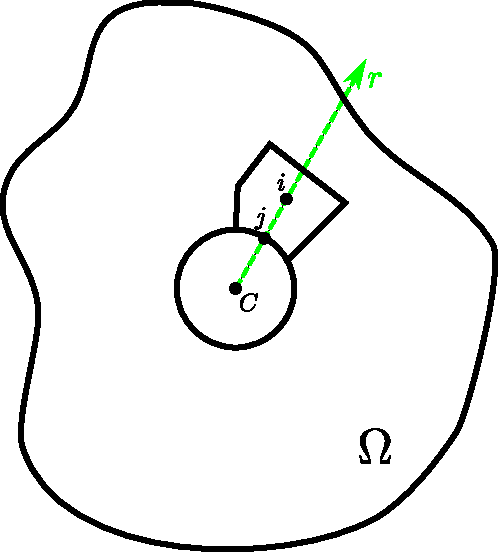
\includegraphics[width=0.4\linewidth]{radial_singularity.pdf}
\caption{Двусвязная область решения}
\label{fig:radial_singularity}
\end{figure}

Возьмём приграничную ячейку $i$ и граничную точку коллокации $j$.
Пусть точки $\vec C$, $\vec c_i$, $\vec c_j$ лежат на одной прямой. Координату
вдоль этой прямой будем называть $r$.
Будем считать, что граничное значение на внутреннем круге
сильно отличается (в большую или меньшую сторону) от
характерного значения $u$ в области расчёта.
Тогда в некотором приближении
решении в окрестности внутреннего круга можно
считать радиально симметричным: зависящим
только от $r$, но не от угла поворота радиус-вектора $\vec r$.
В приближении постоянного коэффициента диффузии такое решение будет удовлетворять уравнению 
\begin{equation*}
\frac 1r \dfr{}{r}\left( r \dfr{u}{r} \right) = 0.
\end{equation*}
Общим решением этого уравнение будет выражение
\begin{equation*}
u = A \ln r + B.
\end{equation*}
Коэффициенты $A$, $B$ выразим через значения
функции в точках коллокации:
\begin{equation*}
u(r_i) = u_i, \quad u(r_j) = u_j.
\end{equation*}
Тогда решение примет вид
\begin{equation*}
u(r) = \frac{\ln r - \ln r_i}{\ln r_j - \ln r_i}\left(u_j - u_i\right) + u_i.
\end{equation*}
Отсюда выразим нормальную производную на грани $\gamma_{ij}$:
\begin{equation} 
\label{eq:fvm_dudn_radial}
\left.\dfr{u}{n}\right|_{\gamma_{ij}} = -\left.\dfr{u}{r}\right|_{r=r_j} =  
\frac {1} {r_j} \, \frac{1}{\ln r_i - \ln r_j}\left(u_j - u_i\right).
\end{equation}
Это выражение будем использовать вместо
\cref{eq:fvm_dudn_dudc} для вычисления производной
на грани с логарифмической особенностью.

Учёт этой особенности можно реализовать за счёт модификации
коэффициента диффузии $\lambda_{ij}$ на граничной грани.
Выражение \cref{eq:fvm_dudn_radial}
можно свести к 
\cref{eq:fvm_dudn_lambda},
если считать диффузию в виде
\begin{equation}
\label{eq:fvm_ln_singularity_hij}
\lambda'_{ij} = \frac{\lambda_{ij}}{r_j} \frac{h_{ij}}{\ln r_i - \ln r_j}
\end{equation}

\subsubsection{Радиально-симметричная постановка}
\label{sec:fvm_radsym}
Теперь рассмотрим уравнение
\cref{eq:poissonnd_lam}
в цилиндрических координатах $(r, \theta, z)$ и радиально-симметричной постановке.
В частных производных определяющее уравнение запишется как
\begin{equation*}
\frac{1}{r}\dfr{}{r}\left( \lambda r \dfr{u}{r} \right) + \dfr{}{z}\left(\lambda \dfr{u}{z}\right) = f, \quad \dfr{u}{\theta} = 0.
\end{equation*}
Заметим, что общий вывод конечнообъёмной схемы
\cref{eq:fvm_lambda_ij_scheme}
использует только формулу Гаусса--Остроградского
\cref{eq:partint_div} в операторном виде.
Поэтому она будет справедлива в любой системе координат.

Особенность выбора радиально-симметричной постановки
проявится только в вычислении площади грани $|\gamma|$
и объёма ячейки $|E|$, которые в этой постановке являются телами
вращения вокруг оси $Oz$.
Вычислим объём как
\begin{equation*}
|E| = \int\limits_{E} d\vec x = \int\limits_0^{2\pi}\left(\iint\limits_{|E|_{rz}} r d r d z\right) d\phi  =
    2\pi \underbrace{\frac{1}{|E|_{rz}}\iint r \, d r d z}_{r_E} \, |E|_{rz} 
\end{equation*}
где $|E|_{rz}$ и $r_E$ -- объём и $r$--координата центра масс ячейки
в декартовой двумерной системе координат $(r, z)$.
Аналогичные рассуждения справедливы и для определения площади грани
через её двумерную площадь $|\gamma|_{rz}$ и центр масс $r_\gamma$.
Тогда окончательно запишем
\begin{equation}
\label{eq:fvm_radsym_measures}
\left|E\right| = 2 \pi r_E |E|_{rz}, \qquad
\left|\gamma\right| = 2 \pi r_\gamma |\gamma|_{rz}
\end{equation}
